\documentclass{article} % For LaTeX2e
\usepackage{nips12submit_e,times}
\usepackage{amsmath}
\usepackage{graphicx}
\usepackage{caption}
\usepackage{subcaption}
\usepackage{comment}
\usepackage{hyperref}
\usepackage[top=1.0in, bottom=1.0in, left=1.0in, right=1.0in]{geometry}

%\renewcommand\refname{Papers To Read}
\title{Semantic Segmentation Using Label Propagation}

\author{
Aravindh Mahendran \\
\texttt{amahend1@andrew.cmu.edu} \\ 
\And
Nitish Thatte \\
\texttt{nitisht@andrew.cmu.edu} \\
\AND
Adwait Gandhe \\
\texttt{agandhe@andrew.cmu.edu} \\
}

\newcommand{\fix}{\marginpar{FIX}}
\newcommand{\new}{\marginpar{NEW}}

\nipsfinalcopy

\begin{document}
\maketitle

\begin{abstract}

\end{abstract}


\section{Introduction}
Semantic segmentation is the process of assigning a class label to each pixel of the image. This is an important problem in computer vision for understanding the underlying information in an image. While classical segmentation techniques group together the pixels based on low level features, semantic segmentation adopts a supervised learning approach. There are two common approaches for semantic segmentation. The first makes use of low level features and combines them with a learning framework to obtain higher level labels. The second approach is to use low level cues, rather than features, with random fields and learn a unified framework using low level segmentation. In this paper, we first estimate the probability for every pixel label pair by using the k-Nearest Neighbors and the Bag of Words model. A Random Forest \cite{Statistics01randomforests} using the color and texton features is trained which decides whether two connected super pixels share a label and the direction in which the label is propagated. 

This paper is structured as follows: Section \ref{sec:Problem} discusses the problem statement. Section \ref{sec:Related} talks about the related work. Section \ref{sec:Proposed} discusses our method for semantic image segmentation. The experiments conducted and the results obtained are presented in section \ref{sec:Exp}. Finally we summarize our conclusions in section \ref{sec:Conclusion}.
\label{sec:Intro}

%------------------------------------------------------------------------------------------

\subsection{Problem Definition}
\label{sec:Problem}

%------------------------------------------------------------------------------------------
\section{Proposed Method}
\label{sec:Proposed}
\subsection{Attempted Methods}
\subsection{Intuition}
\subsection{Our Approach}
\subsubsection{Features}
\paragraph{Textons}
Textons represent texture information.
A collection of filters is used to process each pixel to obtain a per
pixel feature vector.
This is quantized to a single number by selecting a vector nearest to the
current one from a precomputed dictionary.
If each vector in the dictionary is considered to be a word, this
representation gives one word per image pixel and is called the TextonMap
or WordMap. %TODO: Insert figure
A bag of words histogram is computed for each super pixel or segment by
counting word occurrences.
We used the filter bank and dictionary provided by \cite{malisiewicz-cvpr08}.

\paragraph{Color}
Color information is important for separating classes that lack texture or
have similar texture.
We use the per channel color histogram, color mean and standard deviation
from the HSV color space.
\subsubsection{Label Propagation}
\paragraph{Super pixels and connectivity graph}
Each image is divided into super pixels at two different scales such that
the a coarse super pixels align with corresponding finer ones.
This is achieved by using \cite{}.%TODO Cite the super pixel people.
A graph is constructed where each fine super pixel is connected to its
4-connected neighborhood and to all fine super pixels inside the same
coarse super pixel.
We believe that this connectivity helps model non local properties which
are important for determining semantically relevant class labels.

\paragraph{Training the classifier}
We train a classifier that decides whether or not two super pixels should
have the same label.
We assign a label for each super pixel by taking the majority vote over
ground truth labels of each pixel in it.
Each edge in the super pixel graph of a training image is considered a
positive sample if corresponding super pixels have the same label,
negative other wise.
This training data is collected over the k nearest neighbors to the test
image and used to train a random forest.
If done this way, we have too many positive samples and too few negatives
and discriminative learning fails to separate them.
We resample the training data to ensure a low enough ratio between these
before training our classifier.
Note that we train a new random forest for every test image.
Texton and color features are concatenated to describe each super pixel.
Further, each edge in the graph is described by the absolute difference of
their features.

\paragraph{Propagating Labels}
A different segmentation algorithm (see section \ref{baseline}) gives a
probability for each pixel label pair.
The entropy for each super pixel can be calculated from this distribution.
The label with highest probability is treated as the label assigned to
each pixel.
A majority vote over this assignment is used to determine the label for
each super pixel.
When the baseline is inconsistent with the prediction of our random
forest, we propagate labels from the super pixel with higher entropy to
the super pixel with lower entropy.
This propagation is run from the lowest entropy super pixel to the highest
entropy super pixel propagating labels to super pixels further down in
this sorted list.

\subsubsection{Baseline}
\label{baseline}
The label propagation approach discussed above requires per pixel values
for $P(Label)$.
The algorithm which provides this is referred to as baseline and described
below in detail.

\paragraph{Training} Each training image is divided into segments using
Meanshift based EDISON \cite{meanshift}.
A normalized texton histogram (bag of words representation) is computed
for each segment.
The ground truth label for each segment is selected by taking a majority
vote over per pixel ground truth labels.

\paragraph{Testing} For each test image, meanshift segments and normalized
texton histograms of the same are computed.
The probability distribution $P(Label | feature)$ is computed by counting
the occurrences of each label in the K nearest segments from the training
data.
This distribution is copied to each pixel in the image and a per pixel
distribution and entropy is thus available.

\subsection{Related Work}
\label{sec:Related}


%------------------------------------------------------------------------------------------


%------------------------------------------------------------------------------------------
\section{Experiments}
\label{sec:Exp}


\subsection{Description of Experiments}
\label{sec:Description}

We tested our algorithm on the MSRC V1 Dataset \cite{MSRC}, which we randomly into 100 test images and 20 validation images and 100 training images.
Superpixels and connectivity graphs for all the images were precomputed and stored.
Then, we performed leave-one-out cross validation to optimize the parameters in the algorithm. These parameters are $k_{bag}$ for the $k$-nearest-neighbor images from which the bag of words model is computed, $k_{hist}$ for the $k$-nearest-neighbor texton histograms from which the distribution $P(Label | feature)$ is generated, $k_{forest}$ for the $k$-nearest-neighbors used by the random forest, and a ratio parameter used to balanced the number true and false edges on the connectivity graph. Due to a lack of computational resources, optimizing these four parameters simultaneously proved intractable. Therefore, the assumption was made that the parameters for the bag-of-words model and the random forest affect the final segmentation independently. 

Figure \ref{fig:pickK} shows the accuracy of the final segmentations with respect to the parameters for the bag of words model. For this test, the parameters for the random forest, the $k$ value and ratio, were set 11 and 0.8 respectively. We chose a set of parameters that produced a high accuracy that also had low first and second derivatives. We believe low derivatives are desirable as they indicate stability and should generalize well to the test set. Consequently, we chose $k_{bag} = 15$, and $k_{hist} = 7$ as these parameters satisfy both of these requirements.

\begin{figure}[htb]
\centering
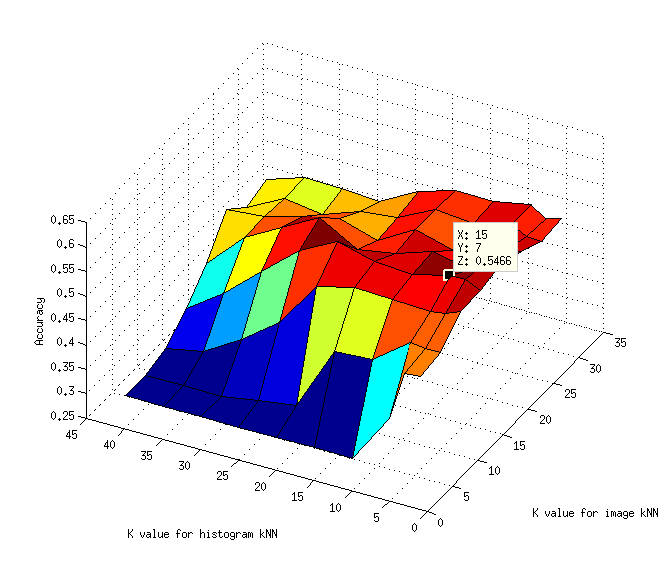
\includegraphics[width = 0.75\textwidth]{./img/pickK_final}
\caption{Results from leave-one-out cross validation on the parameters for the bag of words model. The chosen parameters $k_{imgs} = 15$, and $k_{histo} = 7$ are highlighted.}
\label{fig:pickK}:
\end{figure}


\subsection{Observations}
\label{sec:Observations}

%------------------------------------------------------------------------------------------

\section{Conclusion}
\label{sec:Conclusion}

\bibliographystyle{plain}
\bibliography{final_report}

\end{document}
